\documentclass{beamer}

\usetheme{metropolis}

\usepackage{graphicx}
\usepackage{booktabs}
\usepackage{tikz}
\usepackage{xcolor}

% Updated Green Theme
\definecolor{maingreen}{RGB}{0,153,102}

\setbeamercolor{alerted text}{fg=maingreen}
\setbeamercolor{title}{fg=maingreen}
\setbeamercolor{frametitle}{fg=maingreen}

\setbeamercolor{block title}{bg=maingreen!25,fg=black}
\setbeamercolor{block body}{bg=maingreen!8,fg=black}

\setbeamercolor{alertblock title}{bg=maingreen!40,fg=black}
\setbeamercolor{alertblock body}{bg=maingreen!10,fg=black}

\title{Mini Project Presentation}
\subtitle{Online Canteen Management System}
\author{
Prajit Kumar Singh\\ 
Parth Mishra\\ 
Priyanshu\\ 
Umang Rana\\
Sachlang Debbarma
}
\date{\today}

\begin{document}

%--------------------------------
\begin{frame}
\titlepage
\end{frame}

%--------------------------------
\begin{frame}{Project Overview}

\begin{block}{What is Online Canteen Management System?}
Online Canteen Management System is a web-based platform designed
to simplify food ordering and management in college canteens.
Students can order food online and track their order status.
\end{block}

\begin{columns}

\column{0.48\textwidth}

\begin{alertblock}{Problem}
\begin{itemize}
\item Long queues at canteen
\item Manual order management
\item Delay in food preparation
\end{itemize}
\end{alertblock}

\column{0.48\textwidth}

\begin{block}{Solution}
\begin{itemize}
\item Online food ordering
\item Digital order management
\item Real-time order tracking
\end{itemize}
\end{block}

\end{columns}

\end{frame}

%--------------------------------
\begin{frame}{Technology Stack}

\begin{columns}

\column{0.5\textwidth}

\begin{block}{Frontend}
\begin{itemize}
\item React
\item Tailwind CSS
\end{itemize}
\end{block}

\begin{block}{Backend}
\begin{itemize}
\item Node.js
\item Express.js
\end{itemize}
\end{block}

\column{0.5\textwidth}

\begin{block}{Database}
\begin{itemize}
\item MongoDB
\end{itemize}
\end{block}

\begin{block}{Security \& Deployment}
\begin{itemize}
\item JWT Authentication
\item GitHub
\item Vercel (Frontend)
\item Render (Backend)
\end{itemize}
\end{block}

\end{columns}

\end{frame}

%--------------------------------
\begin{frame}{System Architecture}

\begin{center}
\includegraphics[width=1.1\textwidth,height=0.75\textheight,keepaspectratio]{canteen_architecture.png}
\end{center}

\end{frame}

%--------------------------------
\begin{frame}{System Flow}

\begin{center}

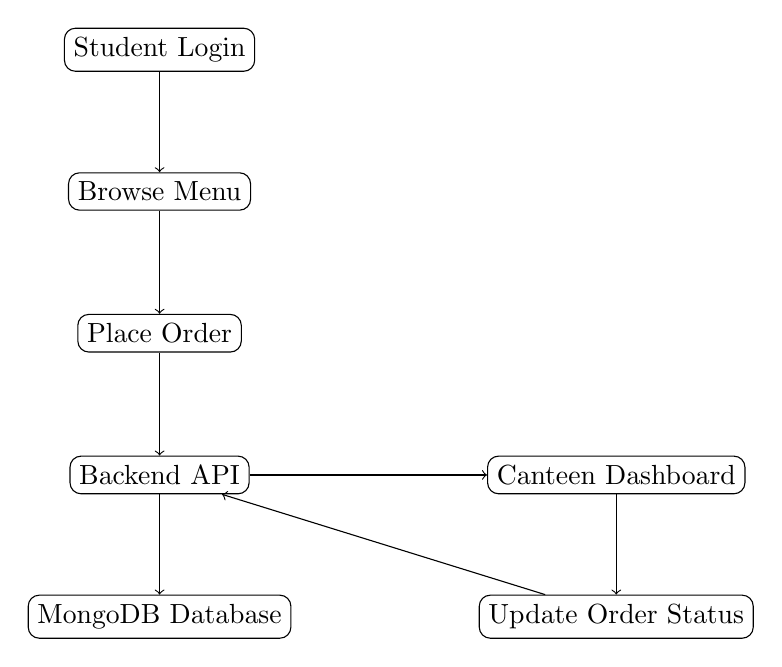
\begin{tikzpicture}[node distance=1.8cm,
every node/.style={draw, rounded corners, align=center}]

\node (login) {Student Login};
\node (menu) [below of=login] {Browse Menu};
\node (order) [below of=menu] {Place Order};
\node (backend) [below of=order] {Backend API};
\node (db) [below of=backend] {MongoDB Database};

\node (admin) [right of=backend, xshift=4cm] {Canteen Dashboard};
\node (update) [below of=admin] {Update Order Status};

\draw[->] (login) -- (menu);
\draw[->] (menu) -- (order);
\draw[->] (order) -- (backend);
\draw[->] (backend) -- (db);

\draw[->] (backend) -- (admin);
\draw[->] (admin) -- (update);
\draw[->] (update) -- (backend);

\end{tikzpicture}

\end{center}

\end{frame}

%--------------------------------
\begin{frame}{Backend API Structure}

\begin{block}{Authentication APIs}
\begin{itemize}
\item POST /register
\item POST /login
\end{itemize}
\end{block}

\begin{block}{Order APIs}
\begin{itemize}
\item GET /menu
\item POST /order/create
\item GET /order/my-orders
\item GET /order/all (Admin)
\item PATCH /order/update-status
\end{itemize}
\end{block}

\begin{block}{Security}
\begin{itemize}
\item JWT based authentication
\item Role-based authorization
\item Password hashing using bcrypt
\end{itemize}
\end{block}

\end{frame}

%--------------------------------
\begin{frame}{Key Features}

\begin{block}{Online Food Ordering}
Students can order food directly from their mobile or laptop.
\end{block}

\begin{block}{Order Tracking}
Students can monitor the status of their food orders in real time.
\end{block}

\begin{block}{Secure Authentication}
JWT-based login system with role verification.
\end{block}

\begin{block}{Admin Dashboard}
Canteen staff can manage incoming orders and update their status.
\end{block}

\end{frame}

%--------------------------------
\begin{frame}{Comparison with Existing Systems}

\begin{center}

\resizebox{\textwidth}{!}{
\begin{tabular}{lccc}
\toprule
Feature & Manual System & Existing Systems & Proposed System \\
\midrule
Food Ordering & Offline & Limited & Online Portal \\
Queue Management & No & Partial & Yes \\
Order Tracking & No & No & Yes \\
Digital Payments & No & Limited & Yes \\
Central Dashboard & No & No & Yes \\
\bottomrule
\end{tabular}
}

\end{center}

\end{frame}

%--------------------------------
\begin{frame}{Project Workflow}

\begin{columns}

\column{0.5\textwidth}

\begin{block}{Planning}
\begin{itemize}
\item Define project objectives
\item Identify system users
\item Analyze canteen management problems
\end{itemize}
\end{block}

\begin{block}{Design}
\begin{itemize}
\item System architecture
\item UI wireframes
\item Database design
\end{itemize}
\end{block}

\column{0.5\textwidth}

\begin{block}{Development}
\begin{itemize}
\item Backend API creation
\item Authentication system
\item Frontend interface development
\end{itemize}
\end{block}

\begin{block}{Deployment}
\begin{itemize}
\item Integrate frontend and backend
\item Deploy using Vercel and Render
\item Connect MongoDB database
\end{itemize}
\end{block}

\end{columns}

\end{frame}

%--------------------------------
\begin{frame}{Project Status}

\begin{columns}

\column{0.5\textwidth}

\begin{block}{Completed}
\begin{itemize}
\item Requirement Analysis
\item System Architecture
\item Database Structure
\end{itemize}
\end{block}

\column{0.5\textwidth}

\begin{alertblock}{In Progress}
\begin{itemize}
\item Backend API Development
\item Order Management System
\item Frontend UI Development
\end{itemize}
\end{alertblock}

\end{columns}

\vspace{0.5cm}

\begin{center}
\textbf{Current Phase: Development}
\end{center}

\end{frame}

%--------------------------------
\begin{frame}{Impact of the System}

\begin{itemize}
\item Reduced waiting time in canteen
\item Faster food service
\item Digital order records
\item Efficient canteen management
\item Improved student experience
\end{itemize}

\end{frame}

%--------------------------------
\begin{frame}{Future Enhancements}

\begin{columns}

\column{0.5\textwidth}

\begin{block}{Smart Features}
\begin{itemize}
\item AI-based food recommendations
\item Automatic order prioritization
\item Smart inventory management
\end{itemize}
\end{block}

\column{0.5\textwidth}

\begin{block}{System Improvements}
\begin{itemize}
\item Real-time notifications
\item Analytics dashboard
\end{itemize}
\end{block}

\end{columns}

\end{frame}

%--------------------------------
\begin{frame}

\centering

\Huge Thank You

\vspace{0.5cm}

\Large Questions?

\vspace{0.7cm}

\small
Online Canteen Management System

\end{frame}

\end{document}